\begin{frame}{Who imagined Data Science first?}
\protect\hypertarget{who-imagined-data-science-first}{}
\includegraphics{images/JamesGray.gif} - Turing Award Winner
\href{https://en.wikipedia.org/wiki/Jim_Gray_(computer_scientist)}{James
Nicholas Gray} - Imagined Data Science as 4rth paradigm of science
\end{frame}

\begin{frame}{What is Data Science?}
\protect\hypertarget{what-is-data-science}{}
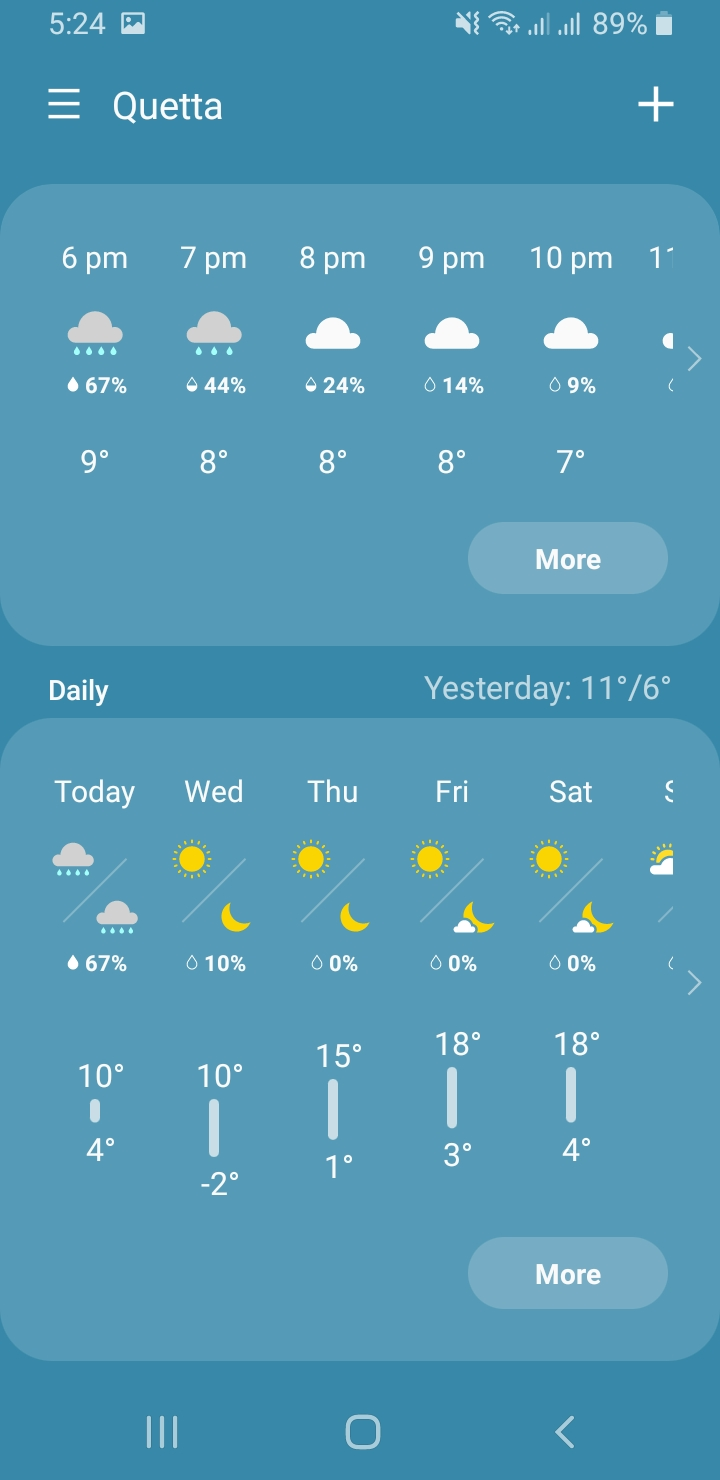
\includegraphics{images/weather.jpeg}
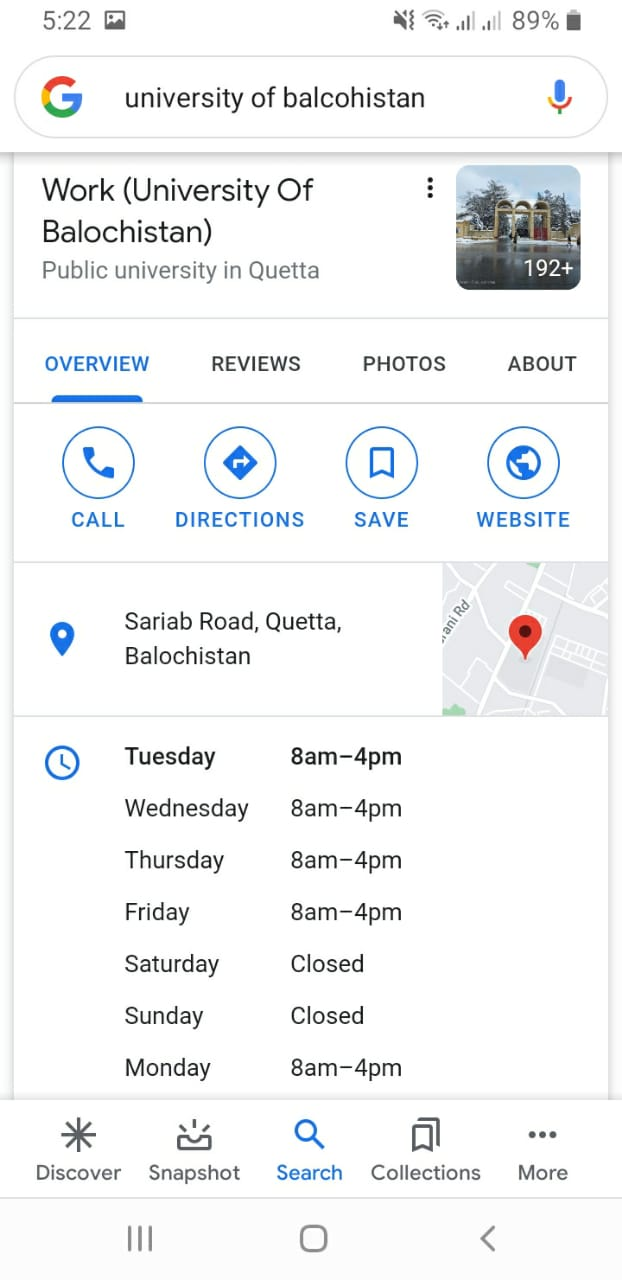
\includegraphics{images/places.jpeg}
\end{frame}

\begin{frame}{What is Data Science?}
\protect\hypertarget{what-is-data-science-1}{}
\begin{itemize}[<+->]
\tightlist
\item
  You have \alert{already experienced} it in \alert{several forms}
\item
  It has been behind resolving some of our common daily tasks for
  several years
\item
  Most of the scientific methods used in data science are not new
\item
  Statistics an old science Simon Laplace 1749 and Thomas Bayes (1701)
\item
  Machine learning relatively new but considered well established
\item
  Computer Science changed lives several decades ago
\end{itemize}
\end{frame}

\begin{frame}{Why Data Science is seen as a novel trend?}
\protect\hypertarget{why-data-science-is-seen-as-a-novel-trend}{}
\begin{itemize}[<+->]
\tightlist
\item
  Datafication: disruptive change in our society caused by the evolution
  of technology
\item
  personal level: list of books, films, food, physical activity,
  purchases
\item
  business level: web activity, network activity, machinery signals
\item
  democratization of data analysis
\item
  large companies Google, Yahoo, IBM, SAS were only players when data
  science had no name
\item
  today the gap between companies and people is shrinking.
\item
  access to cloud computing allows any individual to analyze huge
  amounts of data in short periods of time.

  \begin{itemize}[<+->]
  \tightlist
  \item
    Analytical knowledge is free
  \end{itemize}
\item
  Crucial algorithms needed can be found
\item
  Open source development is the norm
\end{itemize}
\end{frame}

\begin{frame}{Data Science defined}
\protect\hypertarget{data-science-defined}{}
A methodology by which actionable insights can be inferred from data.
\end{frame}

\begin{frame}{Objective of data science}
\protect\hypertarget{objective-of-data-science}{}
\begin{itemize}
\tightlist
\item
  production of beliefs informed by data to be used as the basis of
  decision making
\item
  In absence of data, beliefs are uninformed and decisions are based on
  best practice or intuition.
\end{itemize}
\end{frame}

\begin{frame}{Data Science and 4 strategies}
\protect\hypertarget{data-science-and-4-strategies}{}
\begin{itemize}
\tightlist
\item
  DS allow us to adopt 4 different strategies to explore the world using
  data.
\end{itemize}

\begin{enumerate}
\tightlist
\item
  Probing reality
\item
  Pattern discovery
\item
  Predicting future events
\item
  Understanding people and the world.
\end{enumerate}
\end{frame}

\begin{frame}{Probing Reality}
\protect\hypertarget{probing-reality}{}
\begin{itemize}
\tightlist
\item
  Data can be gathered by

  \begin{enumerate}
  [i)]
  \tightlist
  \item
    passive methods
  \item
    active methods: response of the world to our actions
  \end{enumerate}
\item
  Analysis of these responses can be extremely valuable.

  \begin{itemize}
  \tightlist
  \item
    e.g.~what is the best button size and color? best answer found by
    probing the world.
  \end{itemize}
\end{itemize}
\end{frame}

\begin{frame}{Pattern discovery}
\protect\hypertarget{pattern-discovery}{}
\begin{itemize}
\tightlist
\item
  Datafied problems can be analyzed automatically to discover useful
  patterns.

  \begin{itemize}
  \tightlist
  \item
    e.g.~user profiles an ingredient in programmatic advertising or
    digital marketing.
  \end{itemize}
\end{itemize}
\end{frame}

\begin{frame}{Predicting future events}
\protect\hypertarget{predicting-future-events}{}
\begin{itemize}
\tightlist
\item
  variety of statistical techniques that analyze current and historical
  facts to make predictions about future events.
\end{itemize}
\end{frame}

\begin{frame}{Understanding people and the world}
\protect\hypertarget{understanding-people-and-the-world}{}
\begin{itemize}
\tightlist
\item
  large companies and governments are investing considerable amounts of
  money in research areas e.g.

  \begin{itemize}
  \tightlist
  \item
    understanding natural language

    \begin{itemize}
    \tightlist
    \item
      computer vision
    \item
      psychology
    \item
      neuroscience
    \end{itemize}
  \end{itemize}
\end{itemize}
\end{frame}
